\documentclass[12pt,a4paper]{report}

%adjust your page margins here
\usepackage[top=0.70in, bottom=0.70in, left=0.8in,right=0.80in]{geometry} % setting the page alignment with this package
\usepackage[pdftex]{graphicx} %for embedding images
\usepackage[%dvips, % commented for pdflatex
bookmarks,  colorlinks=false]{hyperref} %for creating links in the pdf version and other additional pdf attributes, no effect on the printed document
\hypersetup{%
    pdfborder = {0 0 0}
}
\usepackage[final]{pdfpages} %for embedding another pdf, remove if not required
\usepackage{float} %used for figure placement with H as a parameter
\usepackage{hyperref}
\usepackage{pslatex} % for times new roman, old package, but works
\usepackage{array} % for making text bold in table
\usepackage{setspace}
\usepackage{float}
\usepackage{enumerate}
\usepackage{longtable}
\usepackage[francais]{babel}
\usepackage{xspace}
\usepackage{pdfpages}
\usepackage[utf8]{inputenc}  
\usepackage[T1]{fontenc}   
\usepackage{listings}
\usepackage[titletoc]{appendix}

\usepackage[font=small,labelfont=bf]{caption}
\def\figurename{\textbf{Figure }}

\usepackage{listings}
\usepackage{color}

\definecolor{dkgreen}{rgb}{0,0.6,0}
\definecolor{gray}{rgb}{0.5,0.5,0.5}
\definecolor{mauve}{rgb}{0.58,0,0.82}
 
\lstset{ %
  language=Java,                % the language of the code
  basicstyle=\footnotesize,           % the size of the fonts that are used for the code
  numbers=left,                   % where to put the line-numbers
  numberstyle=\tiny\color{gray},  % the style that is used for the line-numbers
  stepnumber=1,                   % each line is numbered
  numbersep=5pt,                  % how far the line-numbers are from the code
  backgroundcolor=\color{white},      % choose the background color. You must add \usepackage{color}
  showspaces=false,               % show spaces adding particular underscores
  showstringspaces=false,         % underline spaces within strings
  showtabs=false,                 % show tabs within strings adding particular underscores
  frame=single,                   % adds a frame around the code
  rulecolor=\color{black},        % if not set, the frame-color may be changed on line-breaks within not-black text (e.g. commens (green here))
  tabsize=2,                      % sets default tabsize to 2 spaces
  captionpos=b,                   % sets the caption-position to bottom
  breaklines=true,                % sets automatic line breaking
  breakatwhitespace=false,        % sets if automatic breaks should only happen at whitespace
  title=\lstname,                   % show the filename of files included with \lstinputlisting;
                                  % also try caption instead of title
  keywordstyle=\color{blue},          % keyword style
  commentstyle=\color{dkgreen},       % comment style
  stringstyle=\color{mauve},         % string literal style
  escapeinside={\%*}{*)},            % if you want to add a comment within your code
  morekeywords={*,...}               % if you want to add more keywords to the set
}

%For the header and footer
\usepackage{fancyhdr}
\fancypagestyle{plain}{%
\fancyfoot[L]{\emph{LIPN, Université Paris 13, Villetaneuse}} % except the center
\fancyfoot[R]{\thepage}
\renewcommand{\headrulewidth}{0.4pt}
\renewcommand{\footrulewidth}{0.4pt}
}

\pagestyle{fancy}

\rhead{\emph{ETAMINE}}

\fancyfoot[LO,LE]{\emph{LIPN, Université Paris 13, Villetaneuse}}
\cfoot{}
\fancyfoot[RO, RE]{\thepage}
\renewcommand{\headrulewidth}{0.4pt}
\renewcommand{\footrulewidth}{0.4pt}
%For the header and footer Over

%Page Border
\usepackage{pgf}
\usepackage{pgfpages}

\pgfpagesdeclarelayout{boxed}
{
  \edef\pgfpageoptionborder{0pt}
}
{
  \pgfpagesphysicalpageoptions
  {%
    logical pages=1,%
  }
  \pgfpageslogicalpageoptions{1}
  {
    border code=\pgfsetlinewidth{2pt}\pgfstroke,%
    border shrink=\pgfpageoptionborder,%
    resized width=.95\pgfphysicalwidth,%
    resized height=.95\pgfphysicalheight,%
    center=\pgfpoint{.5\pgfphysicalwidth}{.5\pgfphysicalheight}%
  }%
}
\pgfpagesuselayout{boxed}
\setlength{\parindent}{1cm}
%GLOBAL SETTINGS OVER, DOCUMENT BEGINS
\begin{document}
\renewcommand\bibname{References}
\lhead{ }

%FROM HERE YOUR PAGES START GETTING ADDED

% includes the cover page
\newpage
\begin{center}
\thispagestyle{empty}
\Large{\textbf{RAPPORT DE PROJET\\ \large{SUR}}}\\[0.7cm]
\LARGE{\textsc {\textbf{``RÉFÉRENTIEL ÉTAMINE''}}}\\[0.5cm]
\vspace{0.5cm}
\Large{\textbf{\\Remis à}}
\LARGE{\textbf{\\UNIVERSITÉ DE VILLETANEUSE\\}}
\vspace{1cm}
\Large{\textbf{\\Dans le cadre du module de gestion de projet pour l'obtention du\\}}
\Large{\textbf{\\Master 1\\INFORMATIQUE}}
\vspace{1cm}
\Large{\textbf{\\PAR}}\\[0.5cm]
\begin{table}[h]
\centering
\Large{
\begin{tabular}{>{\bfseries}lc>{\bfseries}r}
Quentin AMELOT\\Paul BAUDOUIN\\Fayize KAIMOU\\Damien LARMINÉ\\Jérémie NIZOU\\Gisio TABERA
\end{tabular}}
\end{table}
\vspace{2.5cm}
\Large{\textbf{UNIVERSITÉ PARIS 13}}\\
\large{\textbf{99 Avenue Jean Baptiste Clément, 93430 Villetaneuse}}
\large{\textbf{\\2014-2015}}\\
\vspace{1cm}
\newpage
\end{center}
\newpage
\pagenumbering{arabic} %reset numbering to normal for the main content
\newpage
\begin{center}
\thispagestyle{empty}
\Large{\textbf{RAPPORT DE PROJET\\SUR}}\\[0.3cm]
\Large{\textsc {\textbf{``RÉFÉRENTIEL ÉTAMINE''}}}\\
\Large{\textbf{\\Remis à}}
\LARGE{\textbf{\\UNIVERSITÉ DE VILLETANEUSE\\}}
\large{\textbf{\\Dans le cadre du module de gestion de projet pour l'obtention du\\}}
\LARGE{\textbf{\\Master 1\\INFORMATIQUE}}
\vspace{0.3cm}
\Large{\textbf{\\PAR}}\\[0.3cm]
\begin{table}[h]
\centering
\Large{
\begin{tabular}{>{\bfseries}lc>{\bfseries}r}
Quentin AMELOT & & Chef de projet\\Damien LARMINÉ & & Responsable Développement\\Fayize KAIMOU & & Développement JAVA\\Gisio TABERA & & Développement PHP\\Jérémie NIZOU & & Responsable Base de données\\
\end{tabular}}
\end{table}
\large{\textbf{SOUS LE TUTORAT DE}}\\
\large{\textbf{M. Michael FORTIER}}\\[0.5cm]

\includegraphics[scale=0.25]{project/images/logo-lipn}\\
\vspace{1.0cm}

\includegraphics[scale=0.25]{project/images/logoUP13}\\
\large{\textbf{99 Avenue Jean Baptiste Clément, 93430 Villetaneuse}}
\large{\textbf{\\2014-2015}}\\[0.5cm]

\newpage

\end{center}
\newpage


% includes the acknowledgements page
\begin{center}
\thispagestyle{empty}
\LARGE{\textbf{Remerciements}}\\[1cm]
\end{center}
\linespread{1.13}
\large{\paragraph{}Nous tenons à remercier \textbf{M. Michael FORTIER} pour son encadrement et son expertise tout
au long du semestre, nous permettant de mener à bien ce projet.}
\large{\paragraph{}Nous tenons également à remercier \textbf{Mr. Lionel POURNIN} ainsi que \textbf{Mr. Nadi TOMEH},
qui, malgré leur travail d'évaluation, ont pris le temps de nous conseiller. Leur implication fut une des clés du bon déroulement de ce projet.
\begin{flushright}
{
Quentin AMELOT\\
Damien LARMINÉ\\
Gisio TABERA\\
Fayize KAIMOU\\
Jérémie NIZOU
}
\end{flushright}
\newpage
 
\newpage

\begin{center}
\thispagestyle{empty}
\vspace{2cm}
\LARGE{\textbf{ABSTRACT}}\\[1.0cm]
\end{center}
\thispagestyle{empty}
\paragraph{}Le but de ce projet était de mettre en place un référentiel de pays, c'est à dire rendre disponible les différentes informations concernant les pays du monde. Ce référentiel devait être implémenté sous la forme d'un WebService JAVA. Afin de rendre l'information encore plus accessible, un client Php ainsi qu'un client JAVA ont été implémentés.}
\paragraph{}Le WebService en lui même se présente sous la forme d'un JAR à éxecuter. Un tomcat intégré permet le déploiement du service. Il est paramétrable grâce à plusieurs fichiers de configuration.
\paragraph{}Le Client JAVA se présente sous la forme d'un code source à intégrer comportant plusieurs méthodes de test. Il dispose de commentaires et d'une Javadoc complète afin de faciliter l'intégration.
\paragraph{}Le Client Php se présente sous la forme d'un site web comportant différentes pages et dont la principale fonction, sous l'onglet "Utiliser Etamine", permet d'interagir avec le WebService.
\paragraph{}Enfin, une application de gestion permet l'interaction avec la base de données du WebService. Elle dispose d'une fonction de login avec mot de passe encrypté. Une fois authentifié, l'utilisateur peut ajouter, supprimer ou modifier des pays de la base de données suivant son niveau d'authentification. % adds the Research Methodology page
\newpage

%To reset the Header & Footer for TOC and LOF
\pagestyle{empty}
\addtocontents{toc}{\protect\thispagestyle{empty}}
\tableofcontents % adds Index Page

\addtocontents{lof}{\protect\thispagestyle{empty}}
\listoffigures % adds List of Figures
\newpage


%And reset back the settings we choose for Header and Footer
\pagestyle{fancy}

\newpage


\chapter{Introduction}
%%%\section{SECTION NAME}
\paragraph{}
Actuellement, il est impossible de trouver rapidement et facilement des informations utiles sur des pays.\\
 Il est obligatoire de faire de longues recherches et les informations récupérées doivent être traitées avant d'être utilisables.\\
L'objectif de ce projet est de développer une solution durable permettant d'en finir avec ces recherches épuisantes et frustrantes en fournissant aux utilisateurs des informations exhaustives, faciles à trouver et surtout directement utilisables.\\
\paragraph{}
Le projet WebService Pays pour Étamine a pour but le développement d'une solution web permettant la mutualisation et l'accès aux données sur les pays du monde entier.\\
La principale application developpée durant ce projet est un WebService permettant de communiquer avec un référentiel des pays contenant des informations utiles comme le code ISO, le libellé ou le taux de change.\\
Les utilisateurs pourront accéder à ces informations par le biais d'un client communiquant avec le WebService et utiliser directement ces informations dans d'autres applications.\\
Une application de gestion est aussi développée pour permettre aux propriétaires de la base de données de pouvoir éditer facilement la base de données et ainsi de l'actualiser. Des scripts pourront ainsi facilement être créés pour automatiser l'actualisation des données.
 % adds the introduction page
\chapter{Spécification des Systèmes Dynamiques}
\section{Technologies utilisées}
\subsection{Maven}
\paragraph{} Maven est un outil de gestion et d'automatisation de projets developpé par la Fondation Apache Software.\\
C'est un outil developpé pour Java, il permet de créer une application à partir de ses sources et d'informations telles que ses dépendances et modules externes.\\
Maven optimise la création et assure le bon déroulement de la fabrication de l'application.\\
Il utilise le paradigme du Project Object Model qui décrit le projet dans un fichier contenant les dépendances, les modules externes, l'ordre de production, le numéro de version, etc...\\
\paragraph{}
Nous avons utilisé cet outil dans le cadre de ce projet car il nous a permis d'optimiser la production des applications dévelopées.\\
Nous avons géneré des sources et centralisé les dépendances et librairies nécessaires grâce à Maven ce qui a permis d'avoir une vision claire du projet et de l'état d'avancement.\\

\subsection{Spring}
\paragraph{} Spring est un framework libre et open-source de développement Java sous licence Apache.\\
Spring est considéré comme un conteneur léger qui crée et met en relation des objets.\\
Il se base sur trois concepts clés qui sont l'inversion de contrôle,qui donne le contrôle de l'éxécution au framework plutôt qu'à l'application elle-même, la programmation orientée aspect, qui sépare le coeur de l'application des aspects techniques, et une couche d'abstraction.\\ 
\paragraph{}
Nous avons utilisé Spring car c'est un framework très puissant et facilement accessible.\\
Il nous a permis de facilement définir l'infrastructure de nos applications et de gérer tous les objets présents à la création et à l'exécution de ces applications.\\

\subsection{SpringWS}
\paragraph{} Spring Web Services est un produit issu du framework Spring permettant la création de Web services.\\
Ce framework facilite la création et l'utilisation de Web services créés en utilisant le protocole SOAP (voir sous-section SOAP et SoapUI).\\
Comme il est basé sur Spring, Spring-WS crée des web services très flexibles et permet même la mise en place de concepts inspirés de Spring comme l'injection de dépendances.\\
\paragraph{}
Nous avons utilisé Spring-WS pour sa capacité à créer des web services à la fois flexibles et complets mais aussi pour sa facilité d'intégration aux composants Spring déjà présents dans les différents applications.\\
Nous avons ainsi pu réutiliser les différentes configurations et expériences liées à Spring que nous avions déjà pour accélerer la production et la mise en place du web service pays.\\

\subsection{Soap et SoapUI}
\paragraph{} SOAP était l'acronyme de Simple Object Access Protocol, un protocole de Remote Procedure Call (RPC) qui permet d'appeler des méthodes à distances.\\
SOAP permet la transmission de messages entre objets distants à l'aide du protocole HTTP ou SMTP.
Il utilise des métadonnées et est composé de deux parties, une enveloppe contenant des informations sur le message et un modèle de données qui contient les données à transmettre.\\
\paragraph{}
Nous avons utilisé SOAP car c'est un protocole qui est indépendant de la plate-forme et du langage utilisé, ce qui a facilité le développement du web service.\\
\paragraph{}
SoapUI est une application open source qui permet le test de web services utilisant le protocole SOAP.\\
Il permet d'inspecter un web service, de simuler une éxécution et de réaliser des tests fonctionnels.\\
\paragraph{}
Nous avons utilisé SoapUI afin de tester notre web service et de localiser les éventuels problèmes de conception ou d'éxécution.\\

\subsection{JAXB}
\paragraph{} JAXB est l'acronyme de Java Architecture for XML Binding, une interface de programmation Java qui permet la création de classes Java à partir d'un fichier XSD et inversement.\\
Grâce à un mapping entre les types XML et Java, il assure la création des classes, de leurs constructeurs ainsi que leurs mutateurs et accesseurs.\\
\paragraph{}
Nous avons utilisé JAXB car il facilite l'utilisation de XML avec Java grâce à son système de schémas.\\
Le framework Spring se configurant à l'aide de fichiers XML, l'utilisation de JAXB a été encore plus importante afin d'être le plus efficient possible.\\

\subsection{Tomcat}
\paragraph{} Tomcat est un conteneur web (serveur) libre appartenant à la Fondation Apache.\\
En plus d'être un serveur, Tomcat gère les servlets ainsi que les Java Server Pages (JSP).\\
Il a été developpé en Java et est donc indépendant de la plate-forme pour son éxécution.\\
Nous avons utilisé Tomcat car c'est aujourd'hui le serveur HTTP multiplate-forme le plus interessant.\\
De plus Spring intègre directement Tomcat, ce qui a facilité la création et le developpement des applications.\\

\subsection{JDBC}
\paragraph{} JDBC est l'acronyme de Java DataBase Connectivity, une interface de programmation Java permettant la communication entre une application Java et une base de données.\\
Cette API fournit des méthodes pour rechercher et modifier une base de données.\\
Nous avons utilisé JDBC pour la communication entre notre référentiel de pays et notre web service.\\
Sa facilité d'utilisation nous a permis de rapidement mettre en place une liaison sûre entre notre base de données et notre web service.\\

\subsection{JUnit}
\paragraph{}JUnit est un framework de test unitaire pour Java.\\
JUnit utilise un système de TestCase qui contiennent des méthodes de test pour tester une classe et des TestSuite qui permettent d'éxécuter certains TestCase prédéfinis.\\
Il permet ainsi de tester certaines parties précises des application pour détécter d'éventuelles erreurs conceptuelles ou de programmation.\\
Nous avons utilisé JUnit pour tester les différentes classes crées dans l'ensemble des applications developpées.\\
Cela nous a permis d'éviter de trouver des erreurs dans le code vers la fin du développement.\\
\chapter{Analyse des Besoins}
\section{Base de données}
\paragraph{}La base de données est composée de nombreuses informations sur les pays du monde entier.\\
Réunir toutes ces informations est un travail extrêmement compliqué et qui nécessite de chercher sur de nombreux sites différents car les informations ne sont pas centralisées.\\
Notre client, Mr Fortier, possède cependant des scripts permettant de récuperer certaines de ces informations mais pour que cela soit efficace, il était nécessaire de faire un travail d'édition sur la base de données déja existante.\\
Nous avons dû pour cela refaire entièrement la base de données pour permettre l'automatisation de la récuperation des données grâce aux scripts.\\
\section{WebService}
\paragraph{} Le web service est la pierre angulaire de ce projet.\\ 
C'est l'application centrale qui va être la plus utilisée.\\
Il était donc nécessaire de la programmer de la manière la plus propre et la plus efficace possible afin d'éviter des lenteurs à l'exécution ou des erreurs de traitement.\\
\chapter{Plan du Système}
\section{Interactions}
\paragraph{} Le projet est composé d'un web service, d'un client PHP, d'un client Java, d'une base de données et d'une application de gestion.\\
Les clients Java et PHP envoient des requêtes SOAP afin de demander des informations sur des pays.\\
Le web service reçoit les requêtes et les traite en envoyant une requête sur la base de données à l'aide de JDBC.\\
La base de données envoie une réponse et le web service utilise SOAP pour envoyer cette réponse aux clients.\\
L'application de gestion permet à un administrateur de se connecter directement à la base de données pour ajouter, supprimer ou modifier un pays manuellement dans la base de données.\\

\vspace{1.0cm}
\begin{figure}[H]
  \centering
    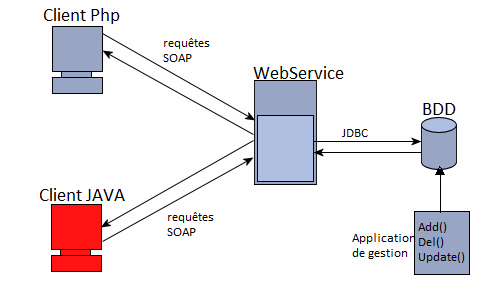
\includegraphics[height= 10cm, width=15cm]{project/images/webservice2}
  \caption{\textbf{Schéma WebService}}
\end{figure}
\chapter{Tests et Assurance Qualité}
\paragraph{} Le projet étant destiné à un public ouvert il était essentiel que les fonctions soient testées, au moins sur les clients et le WebService.
Les tests vérifient les principales fonctionnalités des applications.


\section{Méthodes de test et résultats}
\subsection{Tests du client Java}
\paragraph{} Les méthodes de test du client JAVA servent à tester les différentes réponses du WebService aux différentes requêtes. 
\lstinputlisting[language=Java, firstline=47, lastline=126]{project/code/PaysClientTest.java}

\subsection{Tests du WebService}
\paragraph{} Les méthodes de test du WebService sont principalement liées à la DAO. Elles testent le lien entre les requetes et la Base de Données. 
\lstinputlisting[language=Java, firstline=39, lastline=120]{project/code/TestJDBCWS.java}


\subsection{Tests de l'Application de Gestion}
\paragraph{} Les méthodes de l'Application de Gestion servent à tester les interactions avec la base de donnée comme l'ajout, la suppression ou la modification de pays.
\lstinputlisting[language=Java, firstline=40, lastline=170]{project/code/TestJDBC.java}

\textbf{Note: Les tests doivent s'effectuer manuellement et permettent à l'utilisateur de comprendre le fonctionnement du code}
\chapter{Planification du Projet}
\section{Diagramme de Gantt}
\paragraph{} Au début du projet, nous avions établi un diagramme de Gantt afin de bien organiser le développement des applications du projet.\\
Nous avons suivi précisément ce diagramme de Gantt et nous avons ainsi séparer le temps du projet de la manière la plus efficiente possible.\\
\break
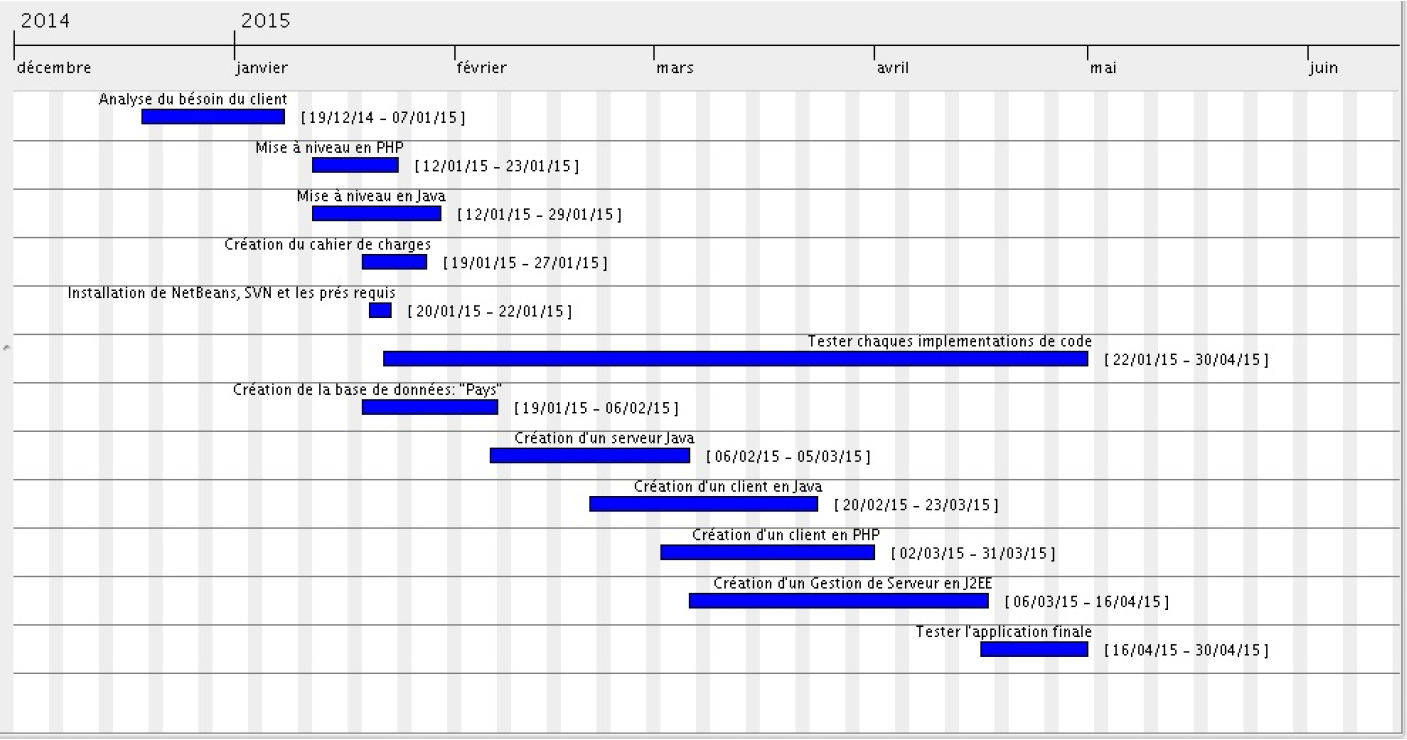
\includegraphics[height= 10cm, width=15cm]{project/images/Image8}

\chapter{Implémentation}
\section{Web Service}
\paragraph{}Le Web Service se lance par le biais de la classe Application.\\
Une fois lancé, le serveur se configure grâce aux éléments de la classe WebServiceConfigPays.\\
Il attend ensuite une requête d'un client, et c'est la classe PaysEndPoint qui traitera cette requête.\\
La classe PaysEndPoint crée un objet PaysRepository et en fonction du type de requête reçu appelle une méthode de cet objet.\\
L'objet Pays Repository charge une fabrique de beans, des objets gérés par Spring et Spring-WS.\\
Cette fabrique est utilisée par la classe IPaysMetier qui crée un objet de type PaysDao et récupère un bean.\\
Elle applique ensuite une méthode de l'objet PaysDao au bean récupéré.\\
La méthode de l'objet PaysDao utilise JDBC pour récuperer les informations nécéssaires dans la base de données.\\
Une fois les informations nécéssaires récupérées, la classe PaysEndpoint renvoie une réponse au client.\\

\section{Client Java}
\paragraph{} Le client se lance à partir de la classe Application.\\
Une fois lancé, il commence à configurer les paramètres nécessaires à la communication avec le web service situé dans la classe PaysConfiguration.\\
Cette classe charge le fichier XML de configuration géré par Spring et Spring-WS et crée un objet PaysClient puis et le renvoie à la classe Application.\\
L'objet PaysClient crée un objet Config qui configurera les paramètres de cet objet PaysClient.\\
La classe application utilise alors l'objet PaysClient récupéré précédemment pour envoyer une requête au web service.\\

\section{Client PHP}
\paragraph{} Le client PHP se présente sous la forme d'un site internet. L'implémentation des fonctions, plus particulièrement celles relatives à SOAP, est détaillée dans la documentation Administrateur. \\
Il constitue l'équivalent du Client Java en php, avec toutefois une interface graphique soignée et un formulaire intuitif pour effectuer les requêtes.

\section{Application de Gestion}
\paragraph{} Une fois l'application de gestion lancé, il est nécessaire de se connecter grâce à un nom d'utilisateur et un mot de passe.\\
La connexion se fait quand l'application crée un objet MainHandler qui va récupèrer un objet paysMetier grâce au fichier de configuration XML géré par Spring et Spring-WS.\\
L'objet paysMetier va créer un objet paysDao et lui appliquer une méthode de recherche d'utilisateur.\\
L'objet paysDao va utiliser JDBC pour chercher dans une base de données spécifiques si le nom d'utilisateur et le mot de passe sont corrects, si c'est le cas, la connexion est validée.
Une fois la connexion effectuée, l'utilisateur peut cliquer sur ajouter, supprimer ou modifier selon son niveau d'autorisation.\\
Quand un ajout, une modification ou une suppression est validée l'application récupère un objet paysMetier grâce au fichier de configuration XML géré par Spring et Spring-WS.\\
Cet objet va créer un objet paysDao et lui appliquer la méthode demandée.\\
L'objet paysDao va utiliser JDBC pour effectuer la méthode demandée et ajouter, modifier ou supprimer un pays dans la base de données.\\


\newpage

 % adds the Project Design
\chapter{Conclusion et Futures Améliorations}
\section{Conclusion}
\paragraph{}Ce projet intéressant et captivant nous aura permis de découvrir et d'apprendre les bases de nombreux frameworks demandés dans le monde du travail pour leur efficacité et leur souplesse. Le module de gestion de projet aura porté notre attention sur des éléments indispensables au bon développement d'un projet comme la documentation ou les contacts réguliers au client pour éviter l'effet tunnel.\\

Ce projet jouant un rôle important dans l'obtention de notre première année de Master, il était nécessaire de choisir le bon projet. A l'unanimité le groupe pense que ce fut le bon choix étant donné qu'il allie nouvelles technologies, programme de deuxième année et une problématique de nature professionnelle.

\section{Futures améliorations}
\paragraph{} Une partie intégrante de chaque projet constitue sa sécurisation quant aux attaques pirates. Trop peu abordée dans ce projet, elle pourrait faire l'objet d'une amélioration future, notamment grâce au module SpringSecurity.\\
Plus de fonctions pourraient également être ajoutées, comme la possibilité de créer des utilisateurs pour l'application de gestion directement en son sein.\\
Une interface graphique plus épurée et moderne pour l'application de gestion sera également à prévoir.\\
Enfin, quelques données supplémentaires pourraient être rajoutées à la base de données.\\ % adds the Scheduling and Planning page
\addcontentsline{toc}{chapter}{Références}
\begin{thebibliography}{99}
\bibitem{docSpring} \url{https://spring.io/docs}
\bibitem{guideSpring} \url{https://spring.io/guides}
\bibitem{docMaven} \url{http://maven.apache.org}
\bibitem{tracLIPN} \url{https://trac.lipn.univ-paris13.fr/projects/pays/}
\bibitem{siteMFortier} \url{https://lipn.univ-paris13.fr/~fortier/Wiki/index.php?n=Accueil.Accueil}
\end{thebibliography} % adds the References page
\begin{appendices}
\chapter{}
\section{\\Cahier des Charges} \label{App:AppendixA}
% the \\ insures the section title is centered below the phrase: AppendixA


\includepdf[pages = 1-15]{project/images/documentation-Cdc}

\newpage
\section{\\Documentation Utilisateur} \label{App:AppendixB}
% the \\ insures the section title is centered below the phrase: Appendix B


\includepdf[pages = 1-13]{project/images/Manuel-utilisation}

\end{appendices} % adds the appendix page

\end{document}